%%%%%%%%%%%%%%%%%%%%%%%%%%%%%%%%%%%%%%%%%%%%%%%%%%%%%%%%%%%%%%%%%%%%%%%%%%%%%%%	
\begin{frame}{Plant Model without control}{Tomato Leaf Curl Virus Disease Using an Epidemiological Model}
		\begin{textblock*}{60mm}(65mm,25mm)
			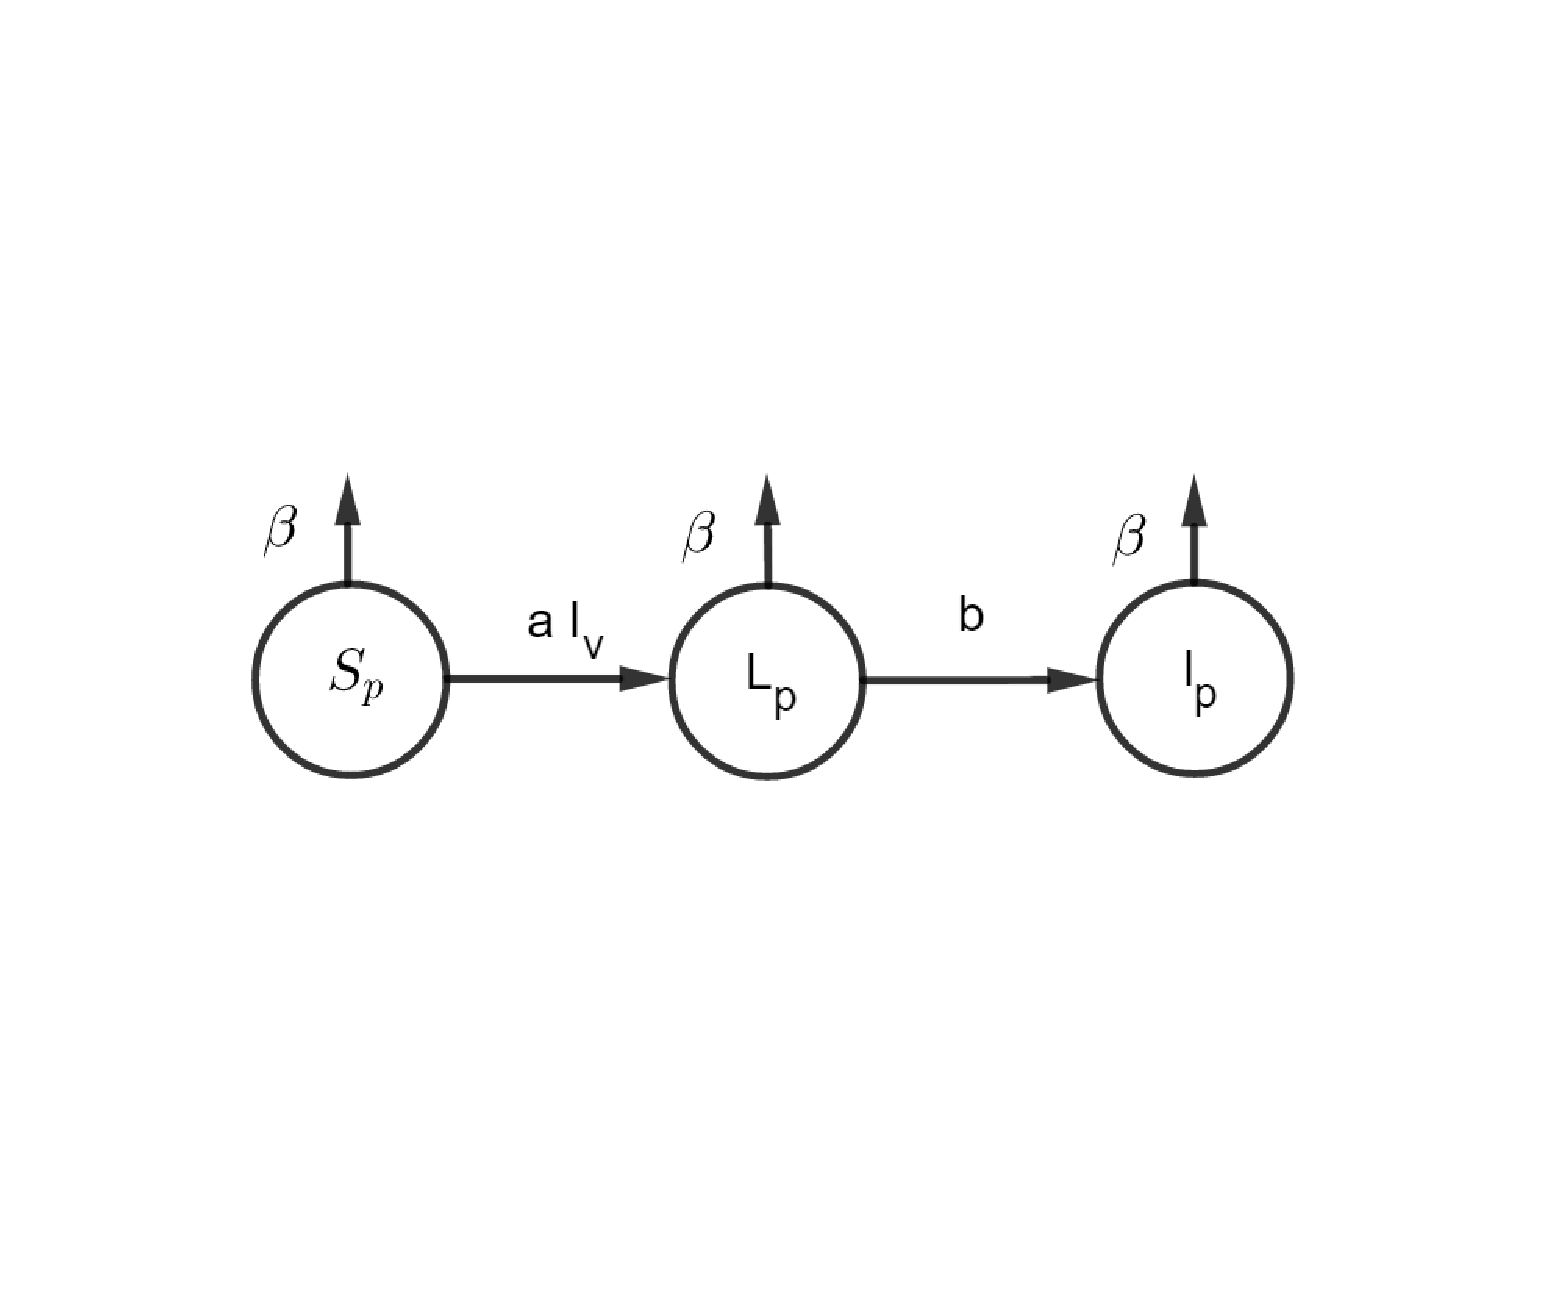
\includegraphics[width=\linewidth]{Feathergraphics/plant_diagram.eps}
		\end{textblock*}
		\begin{textblock*}{60mm}(2mm,25mm)
			\begin{graybox}{Hypothesis:}
				
				\begin{itemize}
					\item Remove from latent and infected plants,
					\item plants become latent plants by infected vectors,
					\item latent plants become infectious plants,
					\item vectors become infected vectors by infected plants,
					\item vectors die per day,
					\item immigration from alternative hosts.
				\end{itemize}
			\end{graybox}	
		\end{textblock*}
\end{frame}
%%%%%%%%%%%%%%%%%%%%%%%%%%%%%%%%%%%%%%%%%%%%%%%%%%%%%%%%%%%%%%%%%%%%%%%%%%%%%%%%
\begin{frame}
		\frametitle{Others Controls}
		\begin{textblock*}{40mm}(2mm,22mm)
			
			\begin{graybox}{Cultural Control}
				\begin{itemize}
					\item<1-> physical barriers,
					\item<2-> planting dates,
					\item<3-> removal of infested plants,
					\item<4-> host plant resistance.
				\end{itemize}
			\end{graybox}
		\end{textblock*}
		
		\begin{textblock*}{40mm}(43mm,22mm)
			\begin{graybox}{Biological control}
				\begin{itemize}
					\item<5-> Parasitoids,
					\item<6-> predators
					\item<7-> fungi.
				\end{itemize}
			\end{graybox}
		\end{textblock*}
		
		\begin{textblock*}{42mm}(85mm,22mm)
			\begin{graybox}{Insecticide}
				\begin{itemize}
					\item<8-> Pymetrozine,
					\item<9-> flupyradifurone,
					\item<10-> cyazypyr.
				\end{itemize}
			\end{graybox}
		\end{textblock*}
		\only<11>
		{
			\begin{textblock*}{90mm}(45mm,47mm)	
				\begin{bibunit}[abbrv]
					\nocite{Shun-xiang2001}
					\putbib
				\end{bibunit}
			\end{textblock*}

			\begin{textblock*}{120mm}(10mm,70mm)
				
				\begin{bibunit}[abbrv]
					\nocite{Smith2014}
					\putbib
				\end{bibunit}
			\end{textblock*}
		}
\end{frame}
%%%%%%%%%%%%%%%%%%%%%%%%%%%%%%%%%%%%%%%%%%%%%%%%%%%%%%%%%%%%%%%%%%%%%%%%%%%%%%%

\begin{frame}{}
	\begin{bibunit}[abbrv]
		\nocite{Holt1999b}
		\putbib
	\end{bibunit}
\end{frame}
%%%%%%%%%%%%%%%%%%%%%%%%%%%%%%%%%%%%%%%%%%%%%%%%%%%%%%%%%%%%%%%%%%%%%%%%%%%%%%%%
\subsection{Model without control}
	\begin{frame}
		\only<1,3>
		{
			\begin{textblock*}{62mm}(2mm,15mm)
				\begin{greenbox}{}
					\begin{align*}
					\frac{dS_p}{dt} &=
					-\beta_p S_p I_v +\textcolor{capri}{r}(L_p +  I_p),\\
					\frac{dL_p}{dt} &= 
					\beta_p S_p I_v -b L_p-\textcolor{capri}{r} L_p,\\
					\frac{dI_p}{dt} &=
					 b L_p - \textcolor{capri}{r} I_p,\\
					\frac{dS_v}{dt} &=
					-\beta_v S_v I_p - \textcolor{cadmiumorange}{\gamma} S_v   +(1-\theta)\mu,\\
					\frac{dI_v}{dt} &=
					\beta_v S_v I_p -\textcolor{cadmiumorange}{\gamma} I_v	+\theta\mu,\\
					S_p(0) &= S_{p_0}, L_p(0) = L_{p_0}, I_p(0) = I_{p_0},\\
					S_v(0) &= S_{v_0}, I_v(0) = I_{v_0}.
					\end{align*}
				\end{greenbox}
			\end{textblock*}
		}
		\only<2>
		{	
			\begin{textblock*}{60mm}(10mm,20mm)
				\begin{tabular}{|c |c |l |} 
					\hline
					Par. & Unit & Descrip. \\ [0.5ex] 
					\hline
					$\beta_p$ & vector$^{-1}$day$^{-1}$ & plants became latently infected rate \\ 
					\hline
					$r$ & day$^{-1}$ &  replanting rate \\
					\hline
					$b$ & day$^{-1}$ & latent class to the infectious class rate\\
					\hline
					$\gamma$ & day$^{-1}$ & vector die or depart rate  \\
					\hline
					$\mu$ & plant$^{-1}$day$^{-1}$ & immigration rate \\
					\hline
					$\theta$ & proportion & proportion of infected vector arrival to crop  \\
					\hline
					$\beta_v$ & plant$^{-1}$day$^{-1}$ & vector infectious acquisition rate\\ 
					\hline
				\end{tabular}
			\end{textblock*}
		}
		\only<3>
		{
			\begin{textblock*}{50mm}(70mm,35mm)
				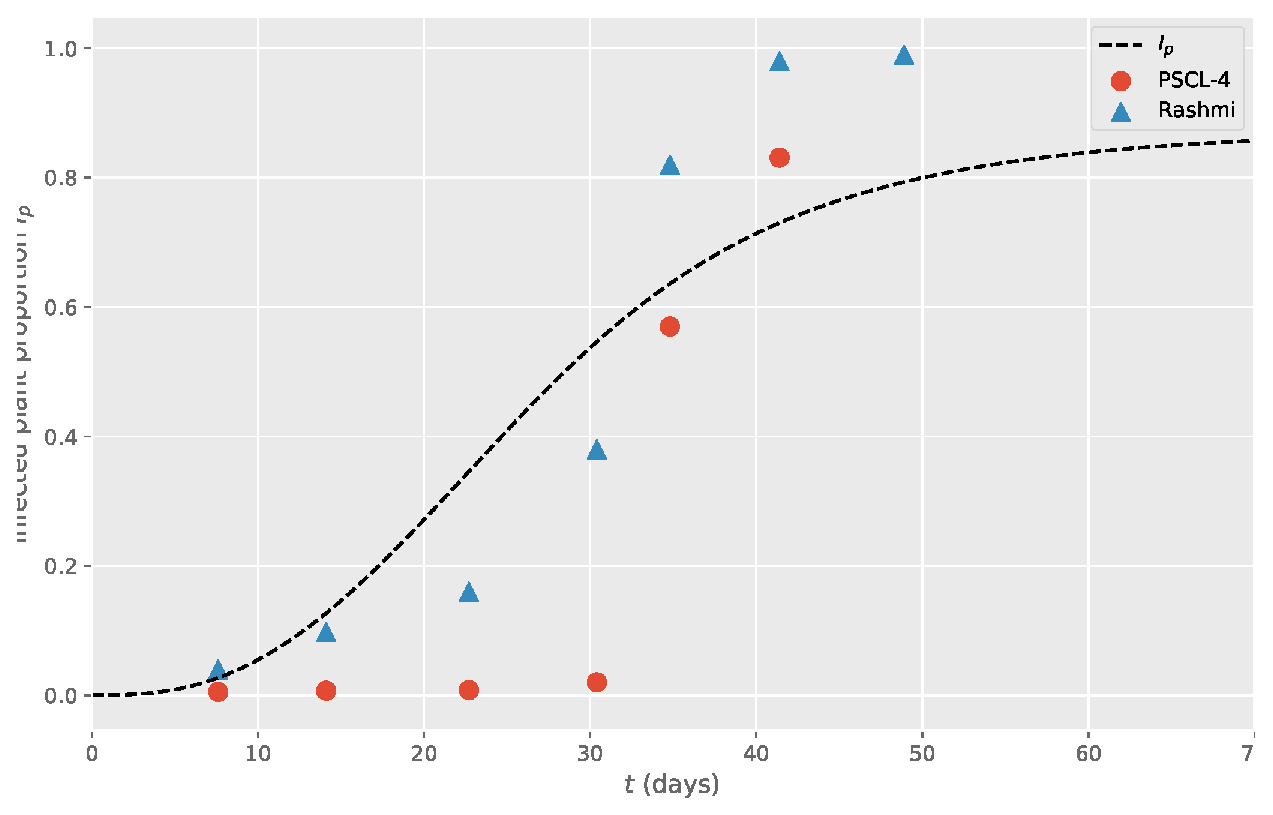
\includegraphics[width=\linewidth]{Feathergraphics/Simulation_data.eps}
			\end{textblock*}
		}
	\end{frame}
%%%%%%%%%%%%%%%%%%%%%%%%%%%%%%%%%%%%%%%%%%%%%%%%%%%%%%%%%%%%%%%%%%%%%%%%%%%%%%%%
	\begin{frame}
	
			\begin{textblock*}{50mm}(5mm,15mm)	
				\only<1,2,3>
				{
				\begin{greenbox}{}
					\begin{equation*}
					R_0=\sqrt{\frac{\beta_v\mu b\beta_p}{r^2(r+b)\gamma}}.
					\end{equation*}
				\end{greenbox}
				}		
			\begin{textblock*}{70mm}(5mm,45mm)
				\begin{yellowbox}{}
				\only<2>
				{	
					If $R_0<1,$
					\begin{equation*}
					\lim\limits_{t\rightarrow \infty}(S_p,L_p,I_p,S_v,I_v)=(N_p,0,0,\frac{\mu}{\gamma},0).
					\end{equation*}
				}
				\only<3>
				{
					If $R_0>1,$
					\begin{equation*}
						\lim\limits_{t\rightarrow \infty}(S_p,L_p,I_p,S_v,I_v)=(S_p^*,L_p^*,I_p^*,S_v^*,I_v^*).
					\end{equation*}
				}
				\end{yellowbox}
			\end{textblock*}
			
			
		\end{textblock*}
		\begin{textblock*}{50mm}(77mm,35mm)
			\only<2>
			{
				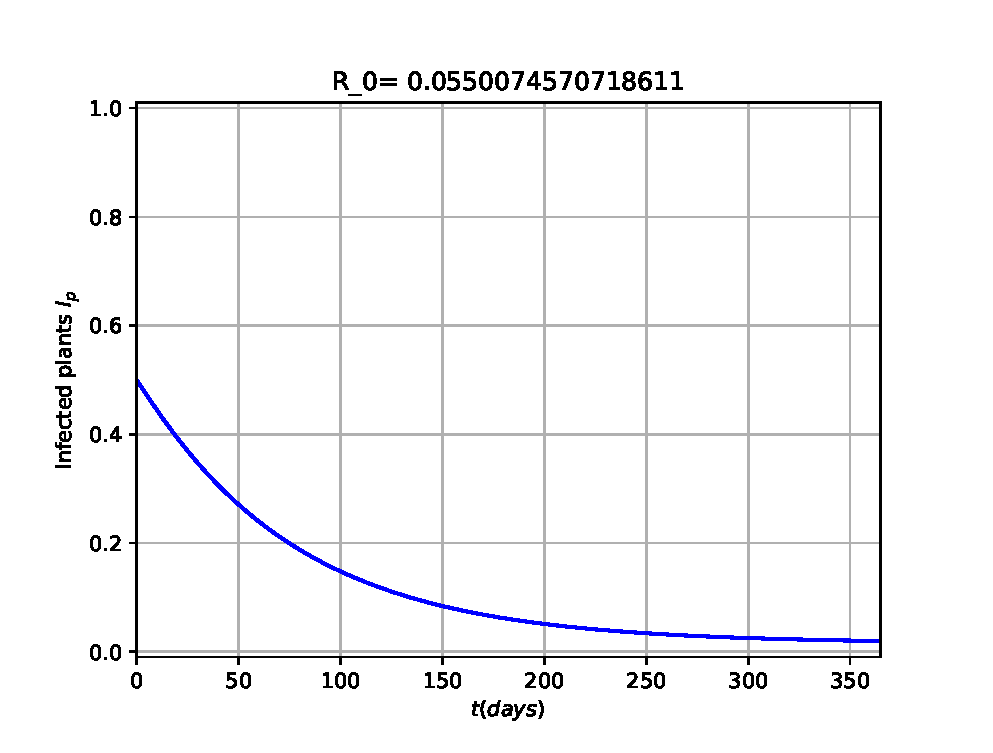
\includegraphics[width=\linewidth]{Feathergraphics/Tomato_simulation_1.eps}
			}
			\only<3>
			{
				\includegraphics[width=\linewidth]{Feathergraphics/Tomato_simulation_2.eps}
			}
		\end{textblock*}	
	\end{frame}
%%%%%%%%%%%%%%%%%%%%%%%%%%%%%%%%%%%%%%%%%%%%%%%%%%%%%%%%%%%%%%%%%%%%%%%%%%%%%%%%
\subsection{Controlled Model}

	\begin{frame}{Plant Model with control}{Tomato Leaf Curl Virus Disease Using an Epidemiological Model}
		\begin{textblock*}{70mm}(1mm,25mm)
			\begin{greenbox}{}
				\begin{align*}
					\frac{dS_p}{dt} &=
					-\beta_p S_p I_v +(\textcolor{capri}{r +u_1})L_p + (\textcolor{capri}{r + u_2}) I_p,\\
					\frac{dL_p}{dt} &=
					\beta_p S_p I_v -b L_p -(\textcolor{capri}{r + u_1})L_p,\\
					\frac{dI_p}{dt} &= 
					b L_p - (\textcolor{capri}{r + u_2}) I_p,\\
					\frac{dS_v}{dt} &=
					-\beta_v S_v I_p - (\textcolor{cadmiumorange}{\gamma+u_3}) S_v +(1-\theta)\mu,\\
					\frac{dI_v}{dt} &=
					\beta_v S_v I_p -(\textcolor{cadmiumorange}{\gamma+u_3}) I_v +\theta\mu,				
				\end{align*}
			\end{greenbox}
		\end{textblock*}
	
		\begin{textblock*}{53mm}(73mm,30mm)
			\begin{yellowbox}{Controls:}
				\begin{itemize}
					\item $u_1$: replanting latent plant,
					\item $u_2$: replanting infected plants,
					\item $u_3$: fumigation.
				\end{itemize}
			\end{yellowbox}
		\end{textblock*}
	\end{frame}
%%%%%%%%%%%%%%%%%%%%%%%%%%%%%%%%%%%%%%%%%%%%%%%%%%%%%%%%%%%%%%%%%%%%%%%%%%%%%%%%
	\begin{frame}[plain]
		\begin{textblock*}{120mm}(2mm,0mm)
			\begin{yellowbox}{OC}
				\begin{align*}
				\min_{\bar{u}(\cdot)\in \tilde{\mathcal{U}}_{x_0}[t_0,T]}J(u_1,u_2,u_3)&=
				\int_{0}^T	(A_1 I_p(t) + A_2 L_p(t) + A_3 I_v(t)
				\\
				&+ c_1 u_1(t)^2 + c_2 u_2(t)^2 + c_3 u_3(t)^2) dt,
				\end{align*}
				s.t.
				\begin{equation*}
					%\left\{ 
					\begin{aligned}
						\frac{dS_p}{dt} &=
						 -\beta_p S_p I_v +(r +u_1)L_p + (r + u_2) I_p,
						 \\
						\frac{dL_p}{dt} &=
						\beta_p S_p I_v -b L_p -(r + u_1)L_p,
						\\
						\frac{dI_p}{dt} &= 
						b L_p - (r + u_2) I_p,
						\\
						\frac{dS_v}{dt} &=
						-\beta_v S_v I_p - (\gamma+u_3) S_v +(1-\theta)\mu,
						\\
						\frac{dI_v}{dt} &=
						\beta_v S_v I_p -(\gamma+u_3) I_v +\theta\mu,
						\\
						&S_p(0) = S_{p_0}, L_p(0) = L_{p_0},
						\\
						&I_p(0) = I_{p_0},S_v(0) = S_{v_0}, I_v(0) = I_{v_0}.
						\end{aligned}%\right.
				\end{equation*}
			\end{yellowbox}
		\end{textblock*}
	\end{frame}
%%%%%%%%%%%%%%%%%%%%%%%%%%%%%%%%%%%%%%%%%%%%%%%%%%%%%%%%%%%%%%%%%%%%%%%%%%%%%%%%
